\documentclass{article}

\usepackage[utf8]{inputenc}
\usepackage[english]{babel}
\usepackage{color}
\usepackage{multicol}
\usepackage{graphicx}
\usepackage{amsfonts}
\usepackage{listings}
\usepackage{color}
\usepackage[justification=centering]{caption}
\usepackage[margin=1in]{geometry}
\definecolor{mygrey}{rgb}{0.99,0.99,0.99}

\title{Digital Clock}
\author{AELLA ABHILASH REDDY (EE16BTECH11001)}
\date{}

\setlength{\columnseprule}{1pt}
\def\columnseprulecolor{\color{white}}

\begin{document}

\maketitle



\section{\textbf{AIM}}
The objective of this project is to make an 24 hour format digital clock using atmega328 and seven segment displays whose time can be set using two potentiometers. 

\section{\textbf{INTRODUCTION}}
Actually here time is displayed on seven segment displays and it is cllaed as digital clock because the power we give to seven segment display is either 0 or 1.



Potentiometer is a device which is equivalent to a rheostat and the speed of rotation or the value of a some display can be altered.

\section{\textbf{PRICIPLE}}
The basic idea of this project is that"MULTIPLEXING".Which means only one of the seven segment display will be give "HIGH" and other will be "LOW"..And the delays of each seven segment displays will be different whose COM pins are given to different digital pins.And the duration between the transition of seven segment display from HIGH  to LOW will be very less which is lessthan minimum perceivance time of naked human eye.


 The time in clock can be changed to required time by using two potentiometers using respective code.And a push button is used to set the time to 00:00:00 at any point of time.

\section{\textbf{Components Required}}
\begin{enumerate}
\item Bread Board
\item Arduino UNO(which contains ATmega 328 chip)
\begin{figure}[htp]
\centering
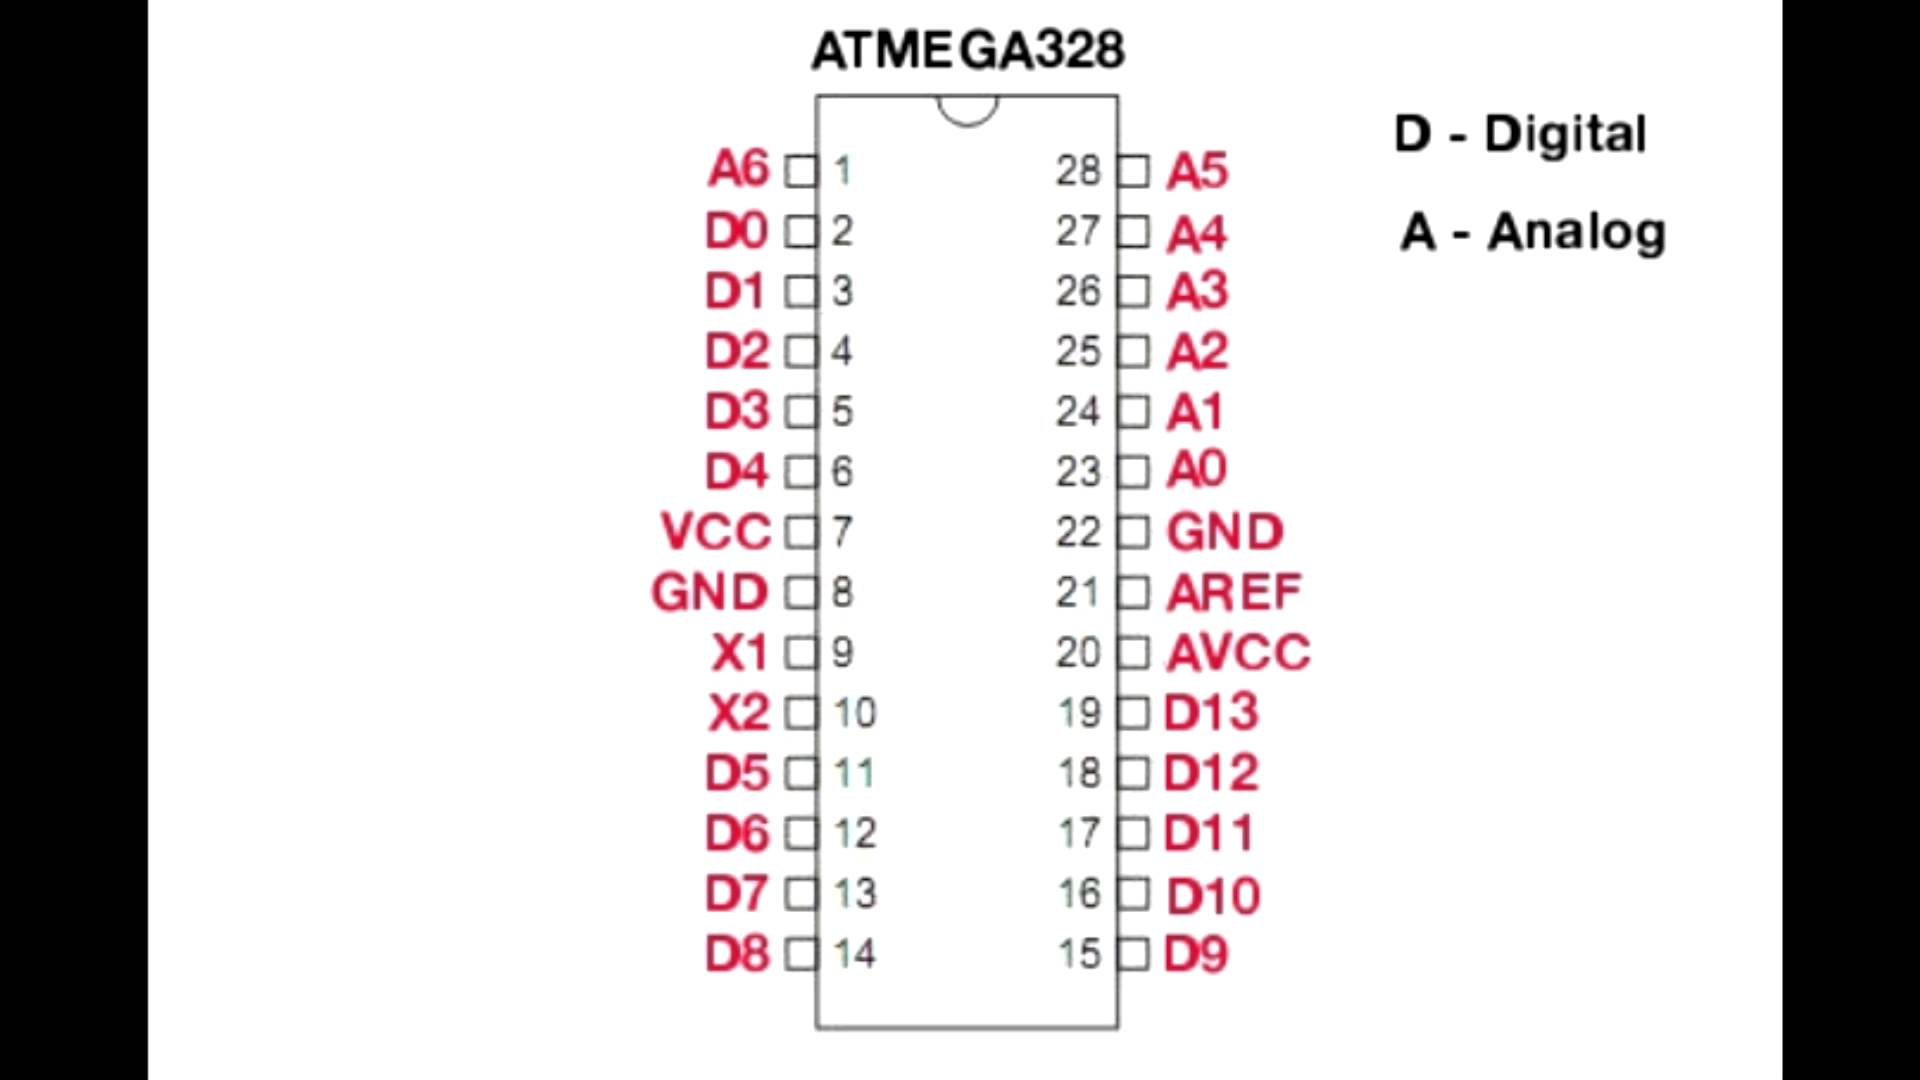
\includegraphics[width=4cm]{atmega}

\caption{atmega328}
\end{figure}

\item 6 Seven segment displays
\item 2 Potentiometers
\begin{figure}[htp]
\centering
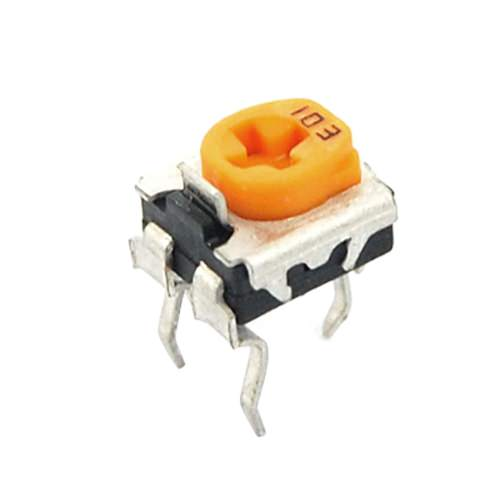
\includegraphics[width=4cm]{potentiometer2}

\label{fig:potentiometer2}
\caption{potentiometer}
\end{figure}
\begin{figure}[htp]
\centering
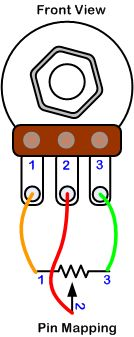
\includegraphics[width=4cm]{potentiometer}
\caption{potentiometer representation}
\label{fig:potentiometer }
\end{figure}
 \item oscillator
\item Push button
\item 6  220 ohm resistors
\item 1 10k ohm resistor
\item 2  220pF capacitors
\end{enumerate}

\section{\textbf{PROCEDURE}}
First clock is tested by arranging circuit on Bread
board.The circuit is arranged such that the COM pins are given to different digital pins of arduino.The a-g pins of displays are short circuited with respective pins of all displays.Two potentiometers are connected to two analog pins.Code is to be uploaded and we can know whether clock is working or not.





If it is working then we have to solder respective components on PCB board.Then we have dump the code in to chip using arduino.Here we have to use oscillator .When we did on bread board we haven't used oscillator because arduino did that. But here we need oscillator to deal with maintaining of frequencies .Power is to be given as per cicuit diagram.After than making an CAD model for dome of clock.
\begin{figure}[htp]
\centering
\includegraphics[width=4cm]{pins}
\caption{pins of atmega328}
\end{figure}
\section{\textbf{CIRCUIT DIAGRAM}}
\begin{figure}[htp]
\centering
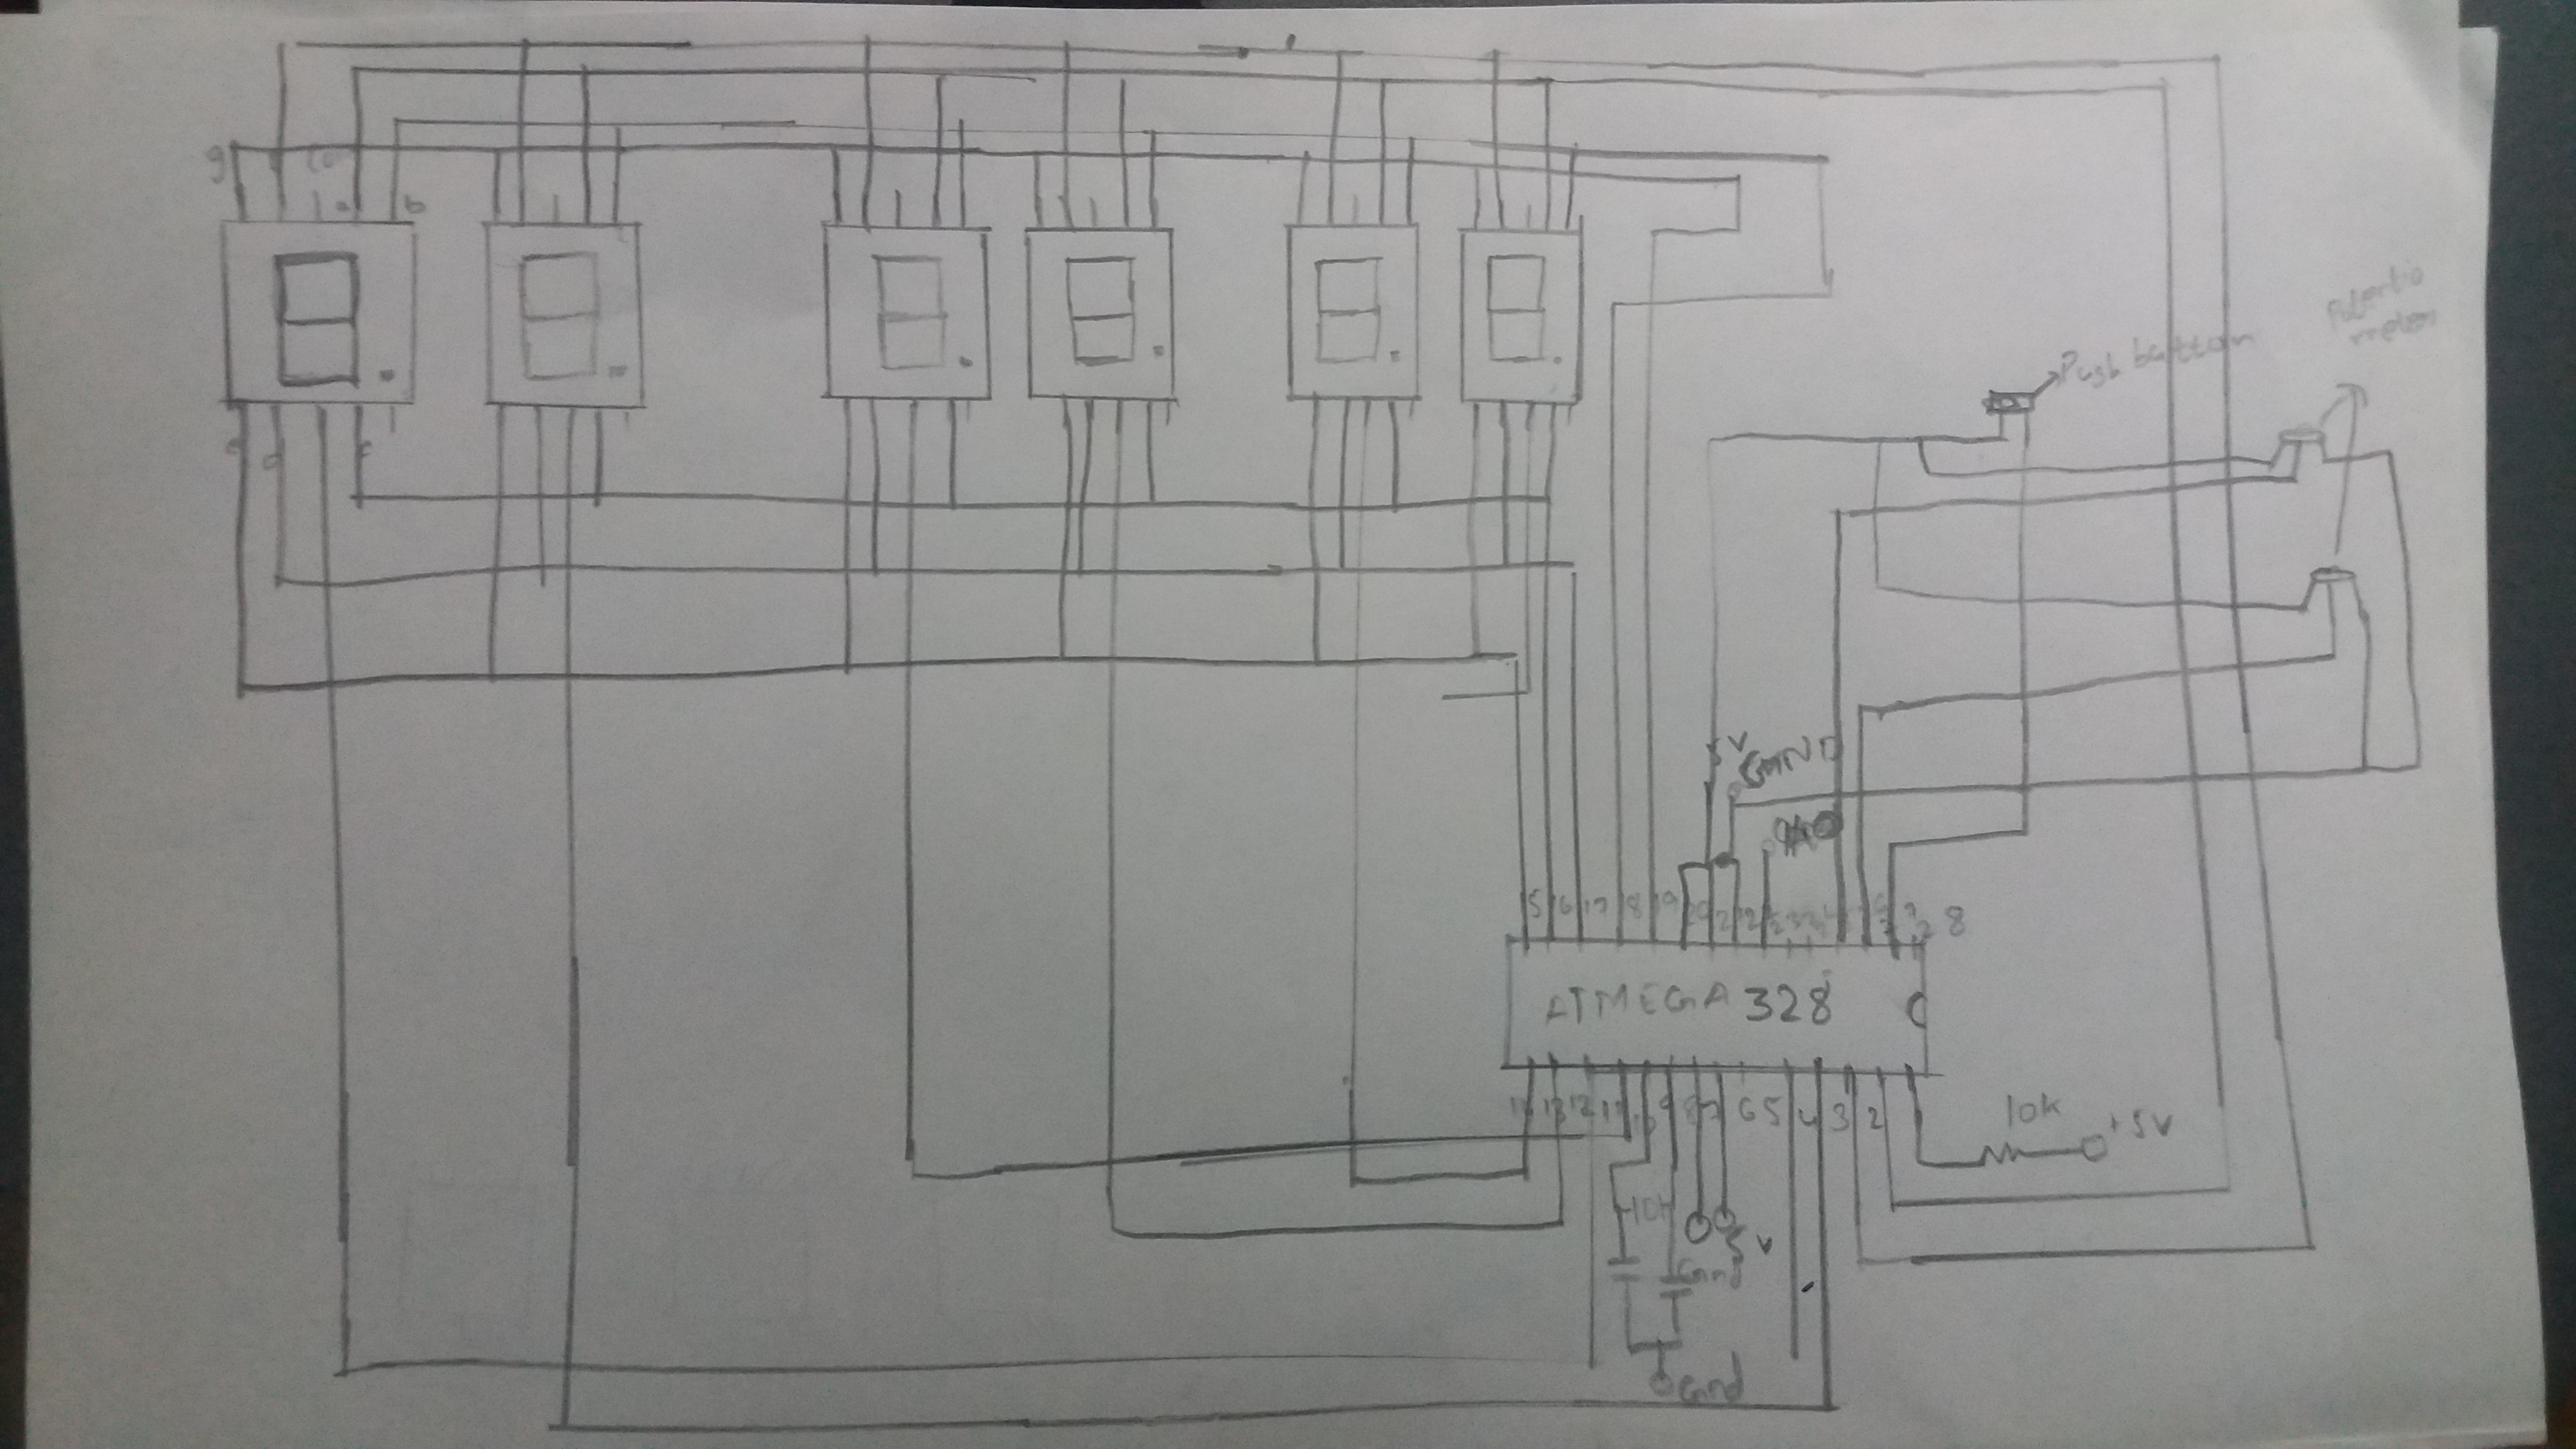
\includegraphics[width=4cm]{circuit}
\caption{circuit diagram}
\label{fig:potentiometer}
\end{figure}


\pagebreak
\section{\textbf{Digital Clock CODE}}
\begin{lstlisting}[frame=single]
int A,B,C,D,a,b,c,d,e,f,g;
int p,q,r,s,t;
long int de=0,dec,mil,pmil=0;
int NM,NH,PM=0,PH=0,pb,pbk=0;
void setup() {
  
 pinMode(0,OUTPUT);
 pinMode(1,OUTPUT);
 pinMode(2,OUTPUT);
 pinMode(3,OUTPUT);
 pinMode(4,OUTPUT);
 pinMode(5,OUTPUT);
 pinMode(6,OUTPUT);
 pinMode(7,OUTPUT);
 pinMode(8,OUTPUT);
 pinMode(9,OUTPUT);
 pinMode(10,OUTPUT);
 pinMode(11,OUTPUT);
 pinMode(12,OUTPUT);
 pinMode(13,INPUT);
}

void display(int y,int Z,int k) 
{
  digitalWrite(7,HIGH);			
  digitalWrite(8,HIGH);
  
  digitalWrite(9,HIGH);			
  digitalWrite(10,HIGH);
  
  digitalWrite(11,HIGH);		
  digitalWrite(12,HIGH);
  A=Z%2;
  Z=Z/2;
  B=Z%2;
  Z=Z/2;
  C=Z%2;
  Z=Z/2;
  D=Z%2;
  
  
  a=!A&&C||A&&!B&&!C&&!D;
  b=!A&&B&&C||A&&!B&&C;
  c=!A&&B&&!C;
  d=A&&!B&&!C||!A&&!B&&C||A&&B&&C;
  e=A||!B&&C;
  f=A&&B||A&&!C&&!D||B&&!C&&!D;
  g=B&&!C&&!D||A&&B&&C&&!D;
  digitalWrite(y,LOW);
  digitalWrite(0,!a);
  digitalWrite(1,!b);
  digitalWrite(2,!c);
  digitalWrite(3,!d);
  digitalWrite(4,!e);
  digitalWrite(5,!f);
  digitalWrite(6,!g);
  while(1)
  {
     mil=millis();
     if(mil-pmil>=k)
     break;
     pb=digitalRead(13);
     if(pb==1)
     {
       pbk=1;
       break;
     }  
  pmil=mil;
  }
 void loop()
 {
  dec=de;
  if(dec==86400)
  de=dec=0;
  int N=analogRead(A1);
 
  NM=((60*N)/1024)*60;
  if(((NM-PM)>=60)||((PM-NM)>=60))
  {
    int K=dec/3600;
    dec=dec+NM;
    if(dec/3600!=K)
    dec=dec-3600;
    de=dec;
  }
  PM=NM;
  int X=analogRead(A2);
  nhr=((24*X)/1024)*3600;
  
   if(((NH-PH)>=3600)||((PH-NH)>=3600))
   {
    dec=(dec+NH)%86400;
    de=dec;
     }
  PH=NH;
  if(pbk==1)
  {
    de=dec=0;
    pbk=0;
  }
    p=dec%10;
    dec=dec/10;
    q=dec%6;
    dec=dec/6;
    r=dec%10;
    dec=dec/10;
    s=dec%6;
    dec=dec/6;
    t=dec%10;
    dec=dec/10;
  for(int n=0;n<125;n++)
  {
    display(12,dec,2);
    display(11,t,2);
    display(10,s,1); 
    display(9,r,1);
    display(8,q,1);
    display(7,p,1);
  }
  de++; 
 }
\end{lstlisting}
\section{Conclusion}
My conclusion is that in this project the important things are 

Getting idea of multiplexing

Coding

Care full soldering with patience



\end{document} 